\chapter{力学性能实验与组织表征}

\section{TC4钛合金的力学实验过程}
力学性能是表征材料性能的重要参数,本实验采用常规的拉伸试验来测量式样的力学性能。测量的包括屈服强度、抗拉强度。

采用拉伸试验机对经固溶时效热处理工艺的试样进行常温微拉伸性能测试,拉 伸速率为2mm/min,每组热处理工艺进行三次测定,取其平均值,微拉伸试样尺寸

在某型号万能力学试验机上测试得到的结果如下:

\begin{table}[htbp]
	\centering
	\caption{\ti 合金的力学性能实验结果}
	\label{sec:mystrength}
		\begin{tabular}{ccc}
			\toprule
			实验编号&$ R_m $/Mpa&$ R_{p0.2} $/Mpa \\
			\midrule
			1 & 950 & 866\\
			2 & 946 & 872\\
			3 & 976 & 884\\
			4 & 988 & 894\\
			5 & 990 & 920\\
			6 & 972 & 886\\
			7 & 966 & 820\\
			8 & 978 & 849\\
			9 & 959 & 836\\
			\bottomrule
		\end{tabular}
\end{table}
\section{TC4钛合金的显微组织表征}
试验期间用来观察组织和分析相结构的检测方法,主要包括光学显微镜 (OM)、扫描式电子显微镜 (SEM)、X射线衍射分析 (XRD)以及透射式电子显微镜 (TEM)等。

将固溶与时效后的试件进行线切割截取显微组织分析试样,截取后的试样进行 150\#、400\#、1000\#、1500\#、2000\#、2500\#金相砂纸磨制,对磨制后的试样采用 0.05umSiO2抛光液在抛光机上进行抛光,去除试样表面的划痕或杂质颗粒,经抛光后的试样采用$ HF:HNO3:H2O=2:4:94 $的Kroll试剂进行腐蚀。腐蚀后的试样分别采用光 学显微镜(OM)、扫描电子显微镜(SEM)对其微观形貌进行观察。


三种不同固溶温度得到的试样组织如下:
\begin{figure}[h!]
	\centering
	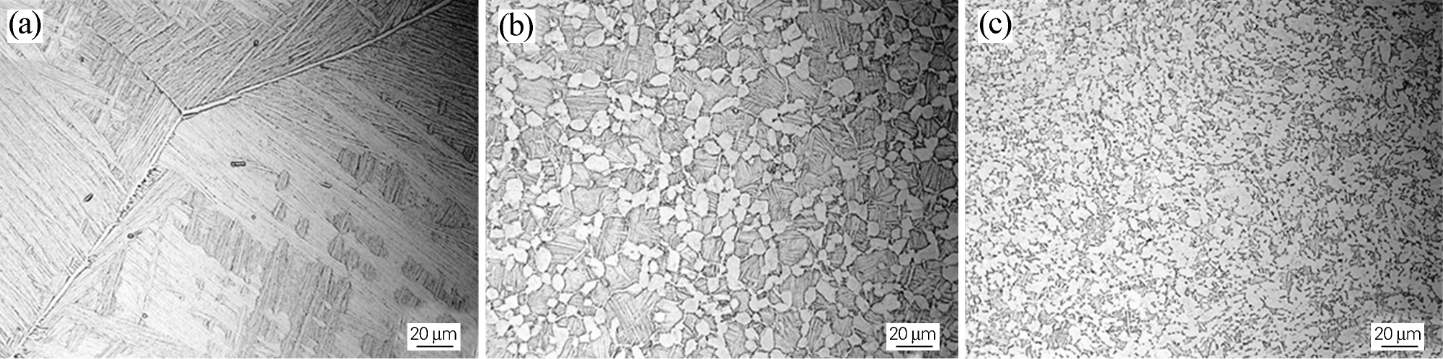
\includegraphics[width=0.7\linewidth]{pic/demo-mico}
	\caption{不同热处理工艺下 TC4 钛合金的显微组织}
	\label{fig:demo-mico}
\end{figure}
\section{结果分析}
本设计采用固溶-时效工艺对合金进行处理。这两种方式对于组织产生的影响如下:

固溶处理的目的是为了使合金在高温状态下内部合金元素发生充分扩散,促使 一定体积分数的 α→β 转变,然后在较快冷却条件下抑制连续冷却过程中 β→α 转变, 从而获得 α′相、α′′相以及 β′相等亚稳定相,为后期的时效处理提供良好的组织状态。 时效处理的目的是通过将固溶处理过程中得到的亚稳定相加热到一定温度进行等温 处理,在热力学的条件下,促使亚稳定相向稳定状态转变,产生细小弥散分布的析 出相,从而对钛合金起到强化作用。

TC4 钛合金在稳定状态下含有少量的 β 相,β 相的存在使其具有热处理强化的能 力。由\ref{fig:tc4change}可知,固溶处理过程中固溶温度对固溶后的亚稳定相种类起决定作 用,不同固溶温度下 α 与 β 相的平衡体积分数不同,造成 β 相中合金元素含量不同, 从而在快速冷却过程中产生不同的亚稳定相。
\begin{figure}[h!]
	\centering
	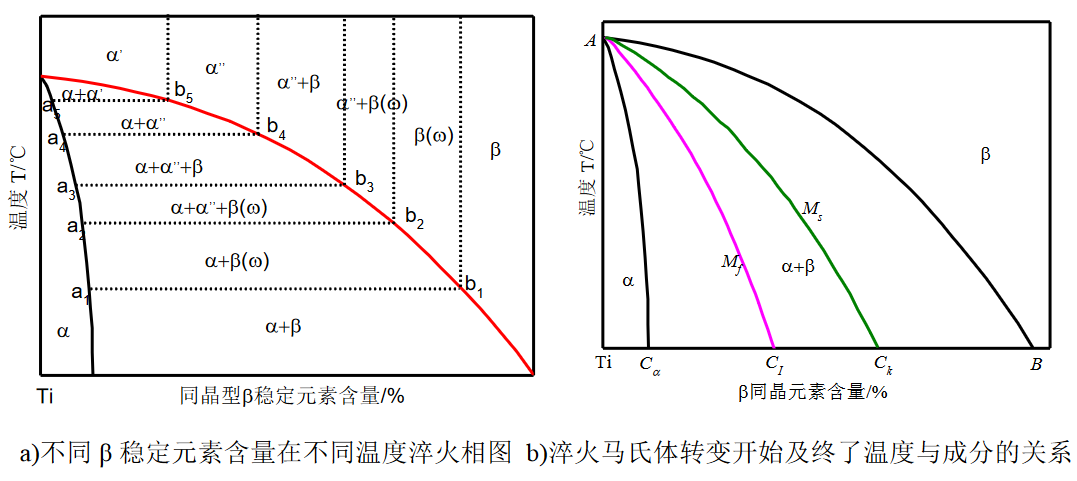
\includegraphics[width=0.7\linewidth]{pic/tc4change}
	\caption{钛合金在淬火过程中的亚稳定相及马氏体转变温度}
	\label{fig:tc4change}
\end{figure}

\subsection{固溶温度对组织性能的影响}
根据金相图可以分析得到,随着固溶温度的提高,抗拉强度先增加后减小,经过固溶时效处理后的TC4钛合金总体上比未经处理的合金力学性能好,固溶温度在950℃(亦即此合金的相变点)附近时,合金的强度最高,
\subsection{冷却方式对组织性能的影响}
对比1与3可得,在水冷的情形下,得到的合金组织中等轴α比较多,合金的强度较好,而油冷处理得到的组织中,α相为充分转化,等轴晶粒较小。
\subsection{时效温度对组织性能的影响}

\subsection{时效时间对组织性能的影响}



\section{小结}